\documentclass[9pt,onecolumn]{article}
\usepackage[paper=a4paper,margin=0.57in]{geometry}
\usepackage[utf8]{inputenc}
\usepackage{graphicx}
\usepackage{hyperref}
\usepackage[labelfont=bf]{caption}
\usepackage{subcaption}
\usepackage{amsmath}
\usepackage{amssymb}
\usepackage{mathtools}
\usepackage{mathrsfs}
\usepackage{physics}
\usepackage[square,numbers]{natbib}
\usepackage[nameinlink,capitalise]{cleveref}
\usepackage{url}
\usepackage{xcolor}
\usepackage{authblk}
\usepackage{rotating}
\usepackage{nameref}
\usepackage{pdflscape}
\usepackage[title]{appendix}
% \usepackage[useregional]{datetime2}
\setlength{\rotFPtop}{0pt plus 1fil}
\setlength\columnsep{.4in}
%\usepackage{tabulary}  
\usepackage[switch, modulo]{lineno}
\linenumbers
\graphicspath{{Fig/Supplement/}}

\makeatletter
\let\@fnsymbol\@arabic
\makeatother
\DeclarePairedDelimiter{\ceil}{\lceil}{\rceil}
\newcommand*\mystrut[1]{\vrule width0pt height0pt depth#1\relax}
\newcommand*\twocell[3]{\begin{tabular}{#1} #2 \\ #3 \end{tabular}}
\newcommand*\threecell[4]{\begin{tabular}{#1} #2 \\ #3 \\ #4 \end{tabular}}
\newcommand*\sfn[2]{$#1 \times 10^{#2}$}
\newcommand*{\intro}{\hyperref[sec:introduction]{Introduction}}

\renewcommand{\thefigure}{S\arabic{figure}}
\renewcommand{\figurename}{Supplementary Figure}

\setcounter{figure}{0}

\setcounter{secnumdepth}{3}
\renewcommand{\thesubsection}{(\alph{subsection})}
    
\begin{document}
\title{Supplement: Improved population fitness in a larger habitat is mostly lost to clonal interference from a zero-sum trait}
\author{Kevin Gomez, Nathan R. Aviles, Jason Bertram, and Joanna Masel}

\maketitle

\newpage
\vspace*{\fill}
\begin{figure}[!h]
    \centering
    \begin{subfigure}[b]{1.0\textwidth}
        \centering
        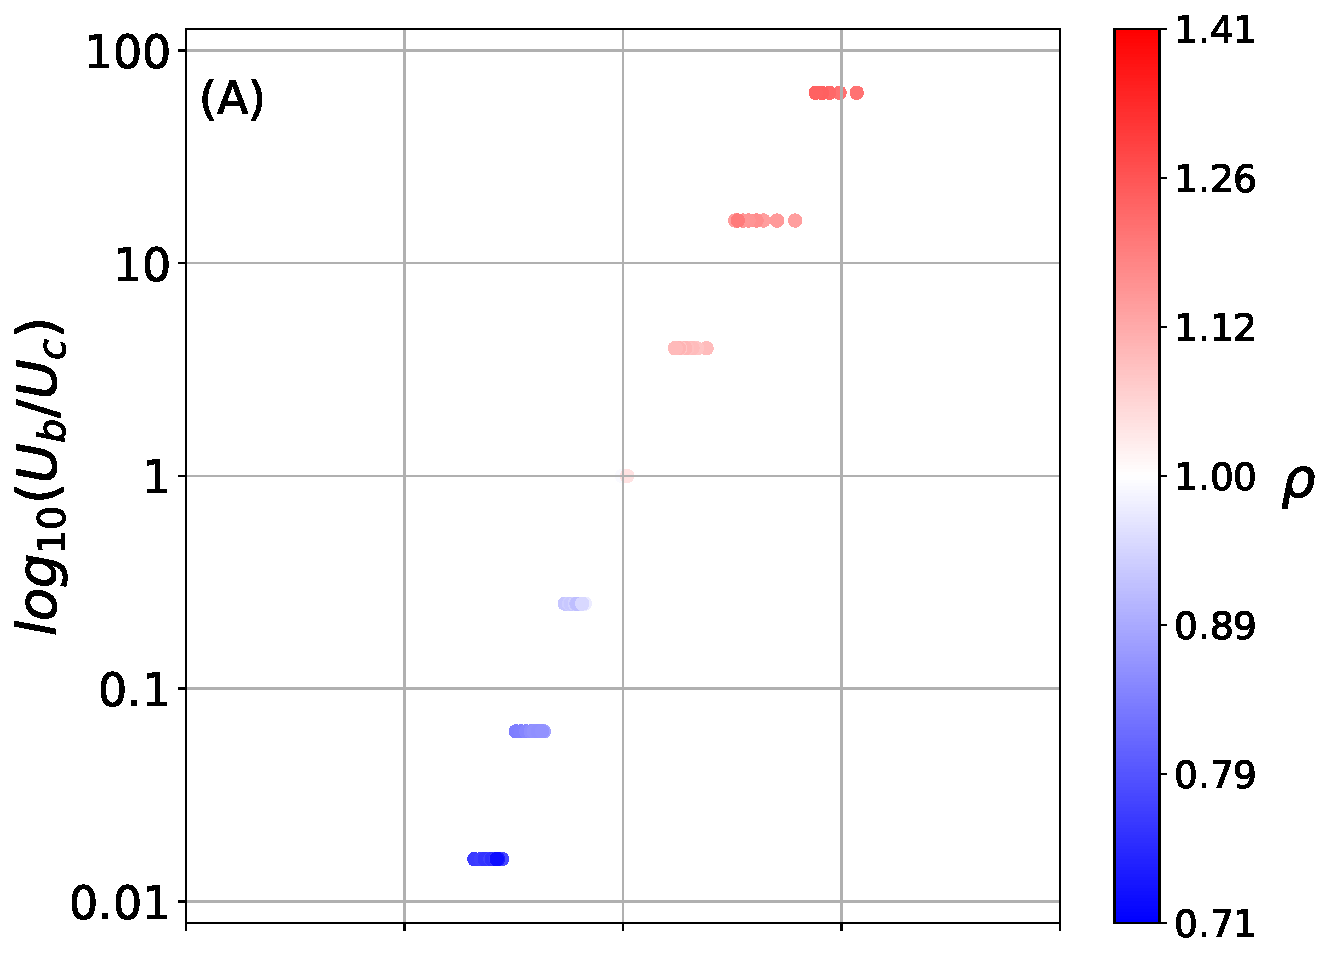
\includegraphics[scale=.5]{fig_bEvo_DRE_Rho_vs_ScSa_UaUc_VaryUaCp_SmallT.pdf}
    \end{subfigure}
    \begin{subfigure}[b]{1.0\textwidth}
        \centering
        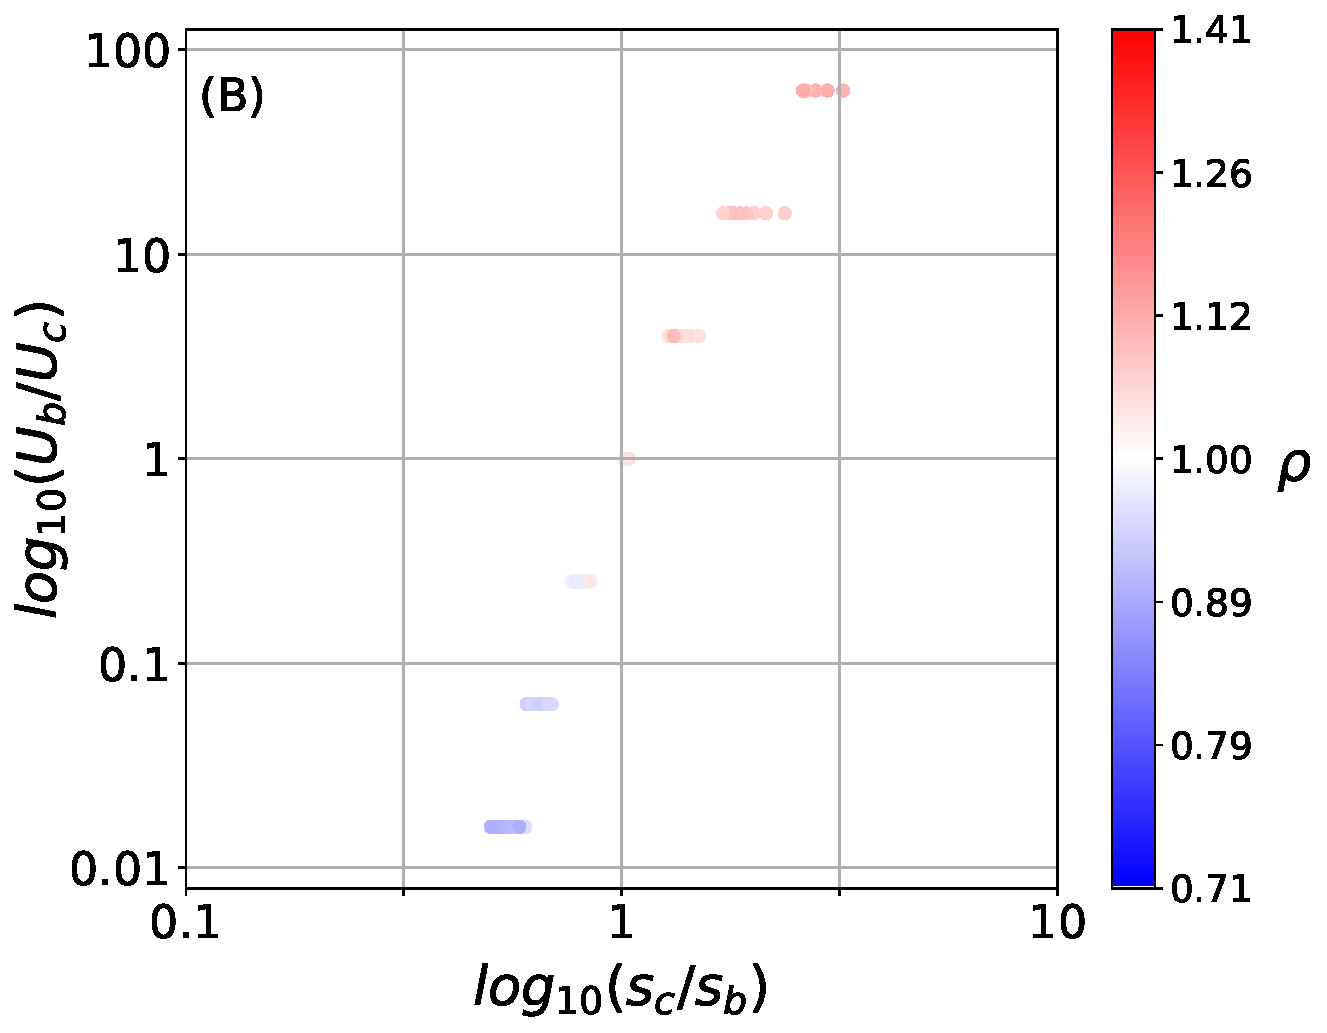
\includegraphics[scale=.5]{fig_bEvo_DRE_Rho_vs_ScSa_UaUc_VaryUaCp_LargeT.pdf}
    \end{subfigure}
    \caption{$\rho$ spans a quantitatively larger range for a smaller number of territories $T=10^7$ (A; $72\% \leq \rho \leq 124\%$) than for $T=10^9$ (Figure 3; $82\% \leq \rho \leq 117\%$) or $T=10^{12}$ (B; $89\% \leq \rho \leq 113\%$). All other parameters are the same as in Figure 3, and results are otherwise similar.}
\label{fig:supp:rho_SmallLargeT}
\end{figure}
\vspace*{\fill}\clearpage

\newpage
\vspace*{\fill}
\begin{figure}[!h]
    \centering
    \begin{subfigure}[b]{1.0\textwidth}
        \centering
        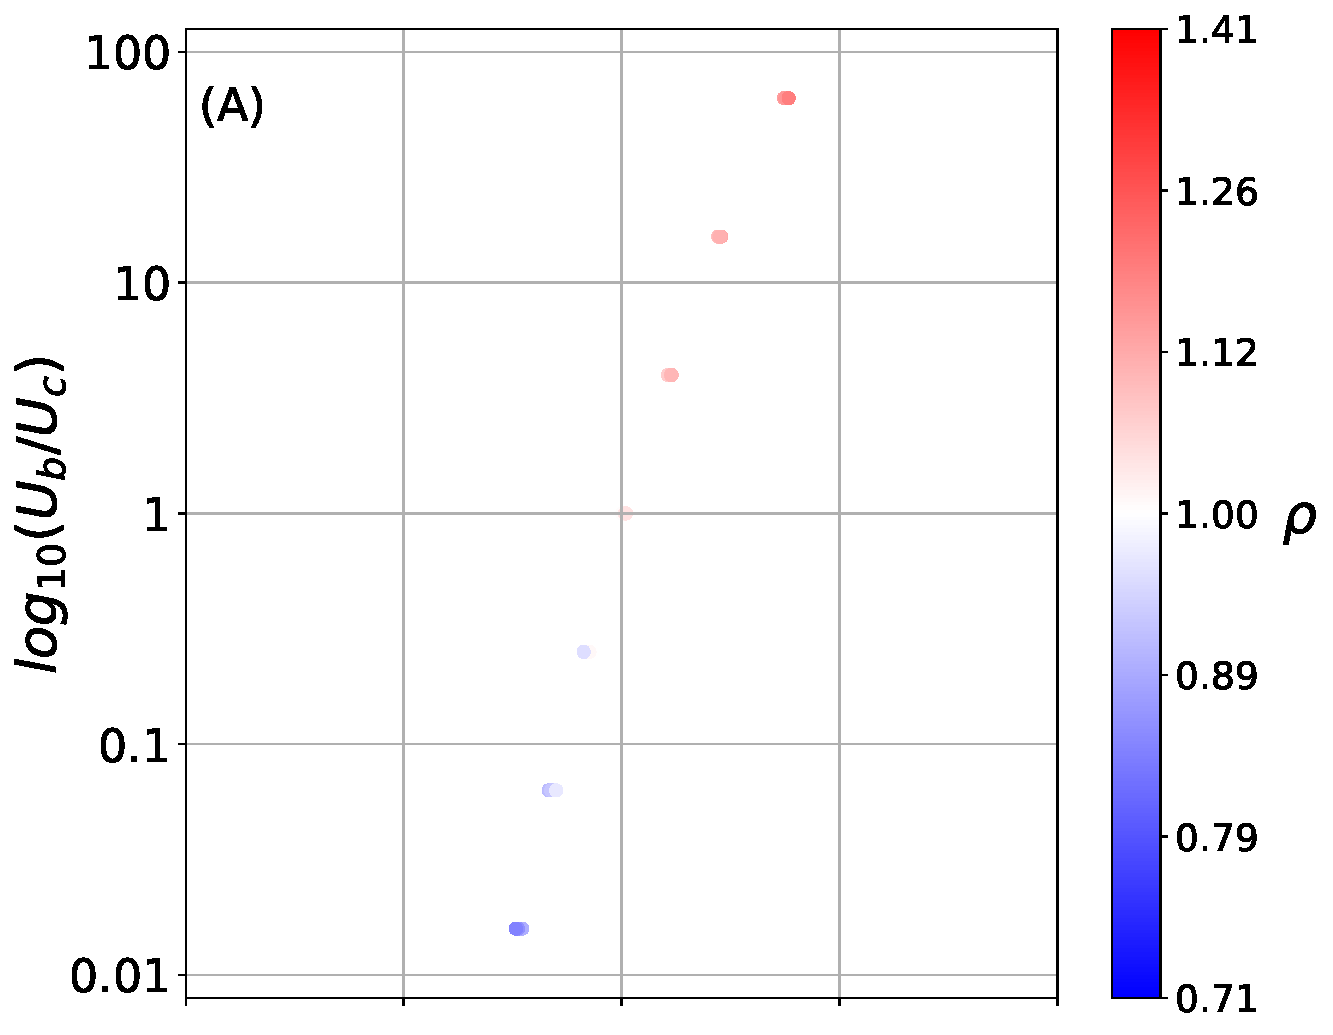
\includegraphics[scale=.5]{fig_bEvo_DRE_Rho_vs_ScSa_UaUc_VaryUaCp_HighAlpha.pdf}
    \end{subfigure}
        \begin{subfigure}[b]{1.0\textwidth}
        \centering
        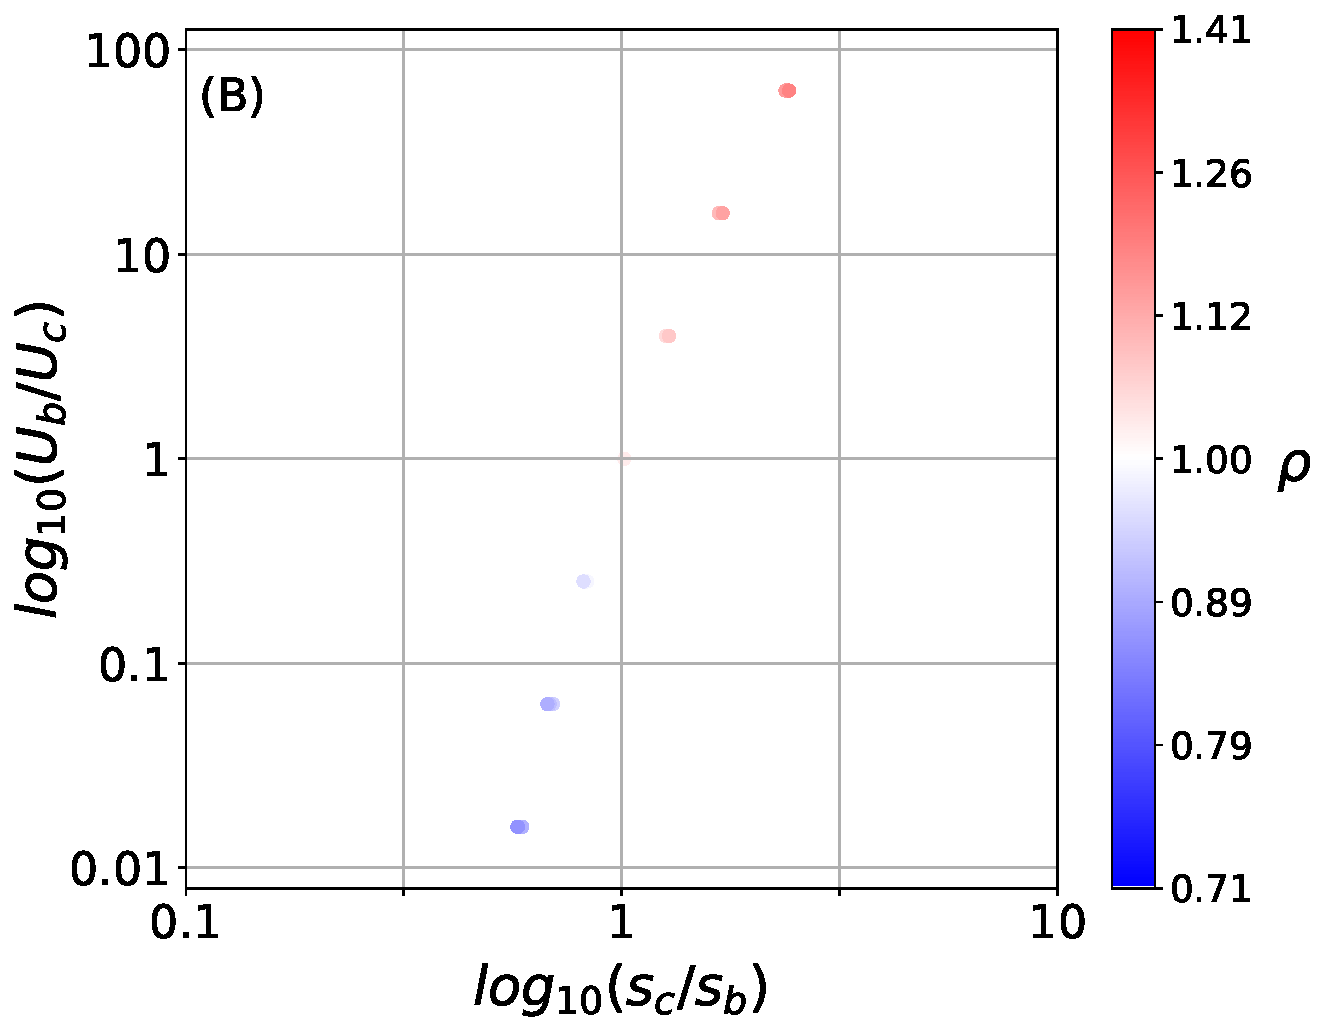
\includegraphics[scale=.5]{fig_bEvo_DRE_Rho_vs_ScSa_UaUc_VaryUaCp_UnbndBVals.pdf}
    \end{subfigure}
    \caption{Weaker diminishing returns epistasis (compared to Figure 3) generates a tighter contour across combinations of $s_c/s_b$ and $U_b/U_c$ as a result of $s_b(x^*)$ being less sensitive to changes in the location of the $v_c(x^*) = v_b(x^*)$ intersection. (A) uses the geometric decay model for selection coefficients ($s_{b,x}=s_{b,1}\cdot \alpha^{x-1}$) with $\alpha=0.9999$ compared to $\alpha=0.99$ in Figure 3. (B) uses an alternative model of diminishing returns epistasis ($s_{b,x}=s_{b,1}\cdot (1+x)^{\alpha-1}$) capable of producing a state space with arbitrarily large $b$ terms. In panel (A), $84\% \leq \rho \leq 120\%$, while in (B), $86\% \leq \rho \leq 119\%$; both ranges are shifted slightly upwards compared to Figure 3 ($82\% \leq \rho \leq 117\%$ with geometrically decaying selection and $\alpha=0.99$). All other parameters are the same as in Figure 3.}
    \label{fig:supp:rho_HighAlpha}
\end{figure}
\vspace*{\fill}\clearpage

\newpage
\vspace*{\fill}
\begin{figure}[!h]
    \centering
    \begin{subfigure}[b]{1.0\textwidth}
        \centering
        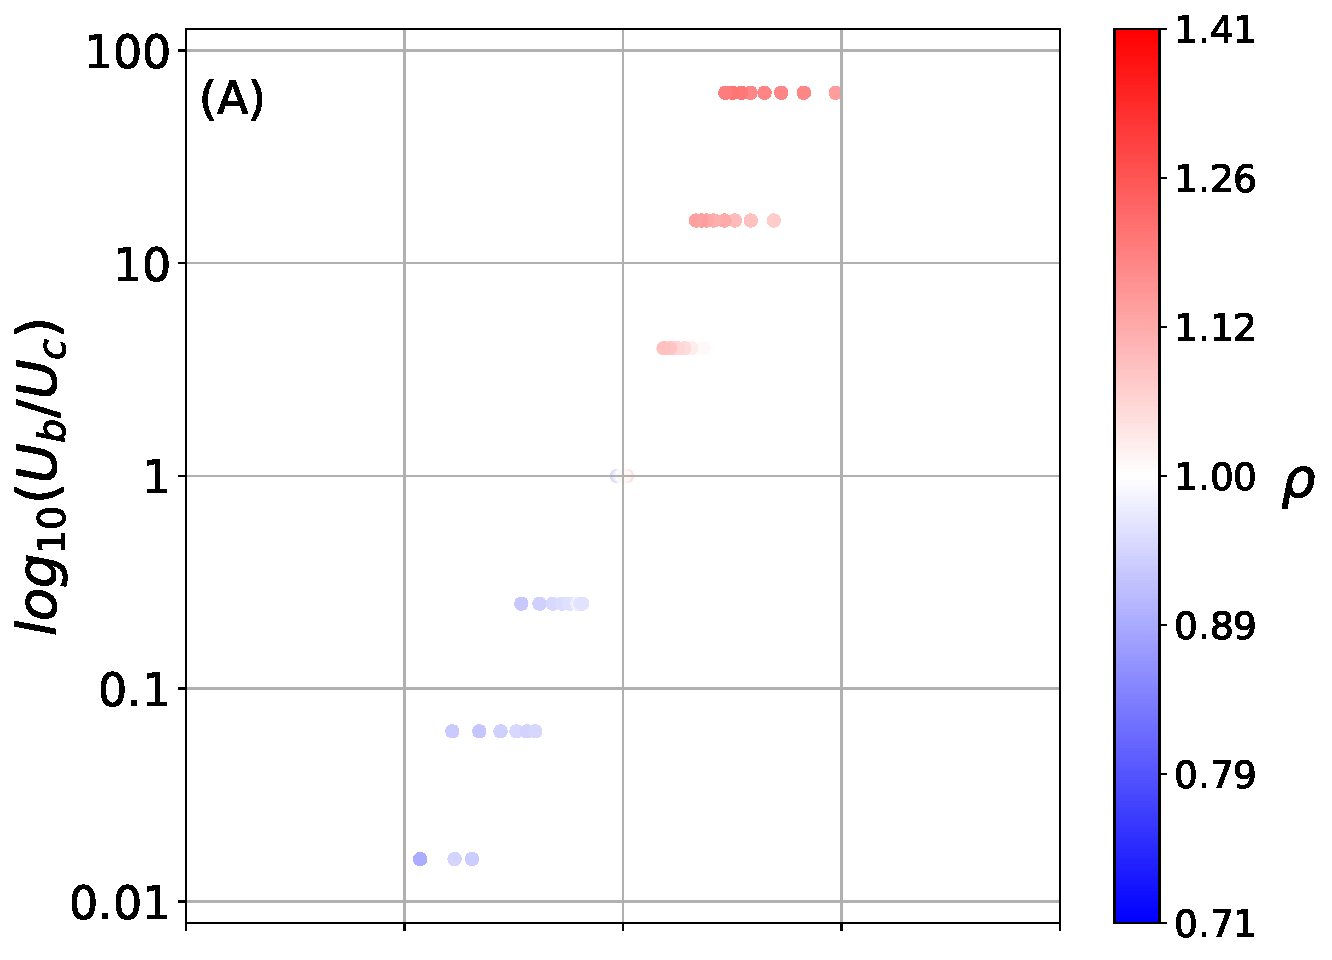
\includegraphics[scale=.5]{fig_bEvo_DRE_Rho_vs_ScSa_UaUc_varyUcSb0.pdf}
    \end{subfigure}
    \begin{subfigure}[b]{1.0\textwidth}
        \centering
        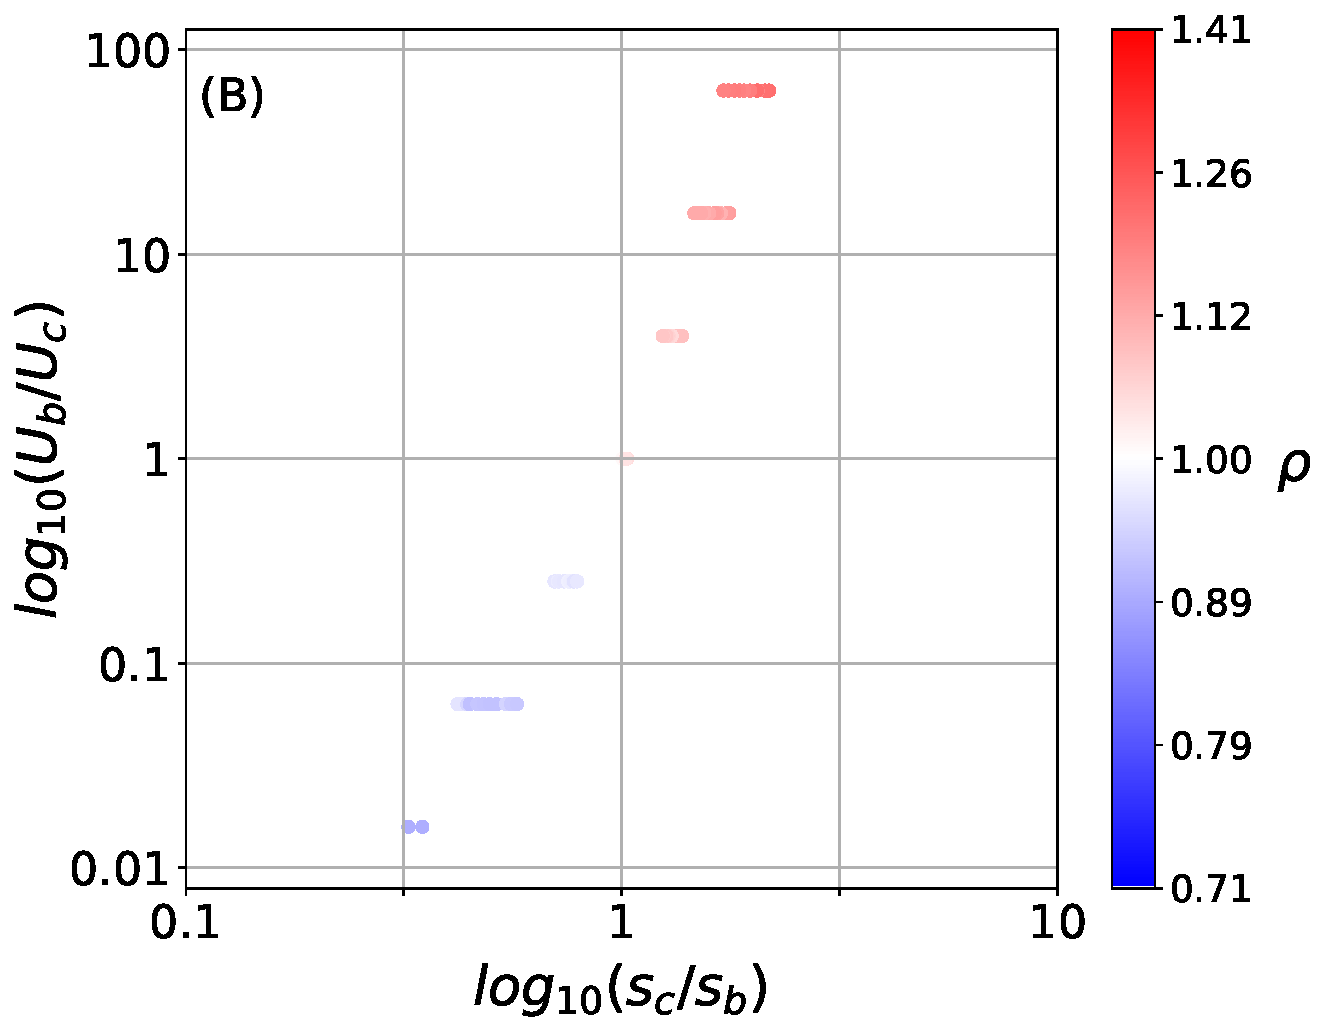
\includegraphics[scale=.5]{fig_bEvo_DRE_Rho_vs_ScSa_UaUc_VaryUcAlpha.pdf}
    \end{subfigure}
    \caption{Results are broadly similar to Figure 3 when instead of varying $U_b$ and $c_+$, we vary $U_c$ and either of the other two absolute fitness model parameters: (A) $s_{b,1}$ and (B) $\alpha$. In panel (A), $\log_{10}(\rho)$ values fall between $89\% \leq \rho \leq 121\%$, while in panel (B), $\rho$ values fall between $89\% \leq \rho \leq 139\%$. In both panels, $T=10^9$, $d=1.2$, $U_b=5\times10^{-6}$, and $c_{+} = 0.44$ are held constant for all points shown above. In (A) we hold $\alpha=0.99$ constant, while in (B) $s_{b,1}=0.02$ is held constant. In (A),  $U_c$-$s_{b,1}$ combinations were formed as an evenly spaced grid on a log scale across the ranges $5.0\times 10^{-9} \leq U_c \leq 5.0\times 10^{-3}$ and $0.002 \leq s_{b,1} \leq 0.2$. In (B), $U_b$-$\alpha$ combinations span an evenly spaced grid on a log scale across the ranges $5.0\times 10^{-9} \leq U_b \leq 5.0\times 10^{-3}$ and $0.9675 \leq \alpha \leq 0.9992$.}
    \label{fig:supp:rho_VaryUcSb0_VaryUcAlpha}
\end{figure}
\vspace*{\fill}\clearpage

\newpage
\begin{landscape}
\vspace*{\fill}
\begin{figure}[!h]
    \centering
    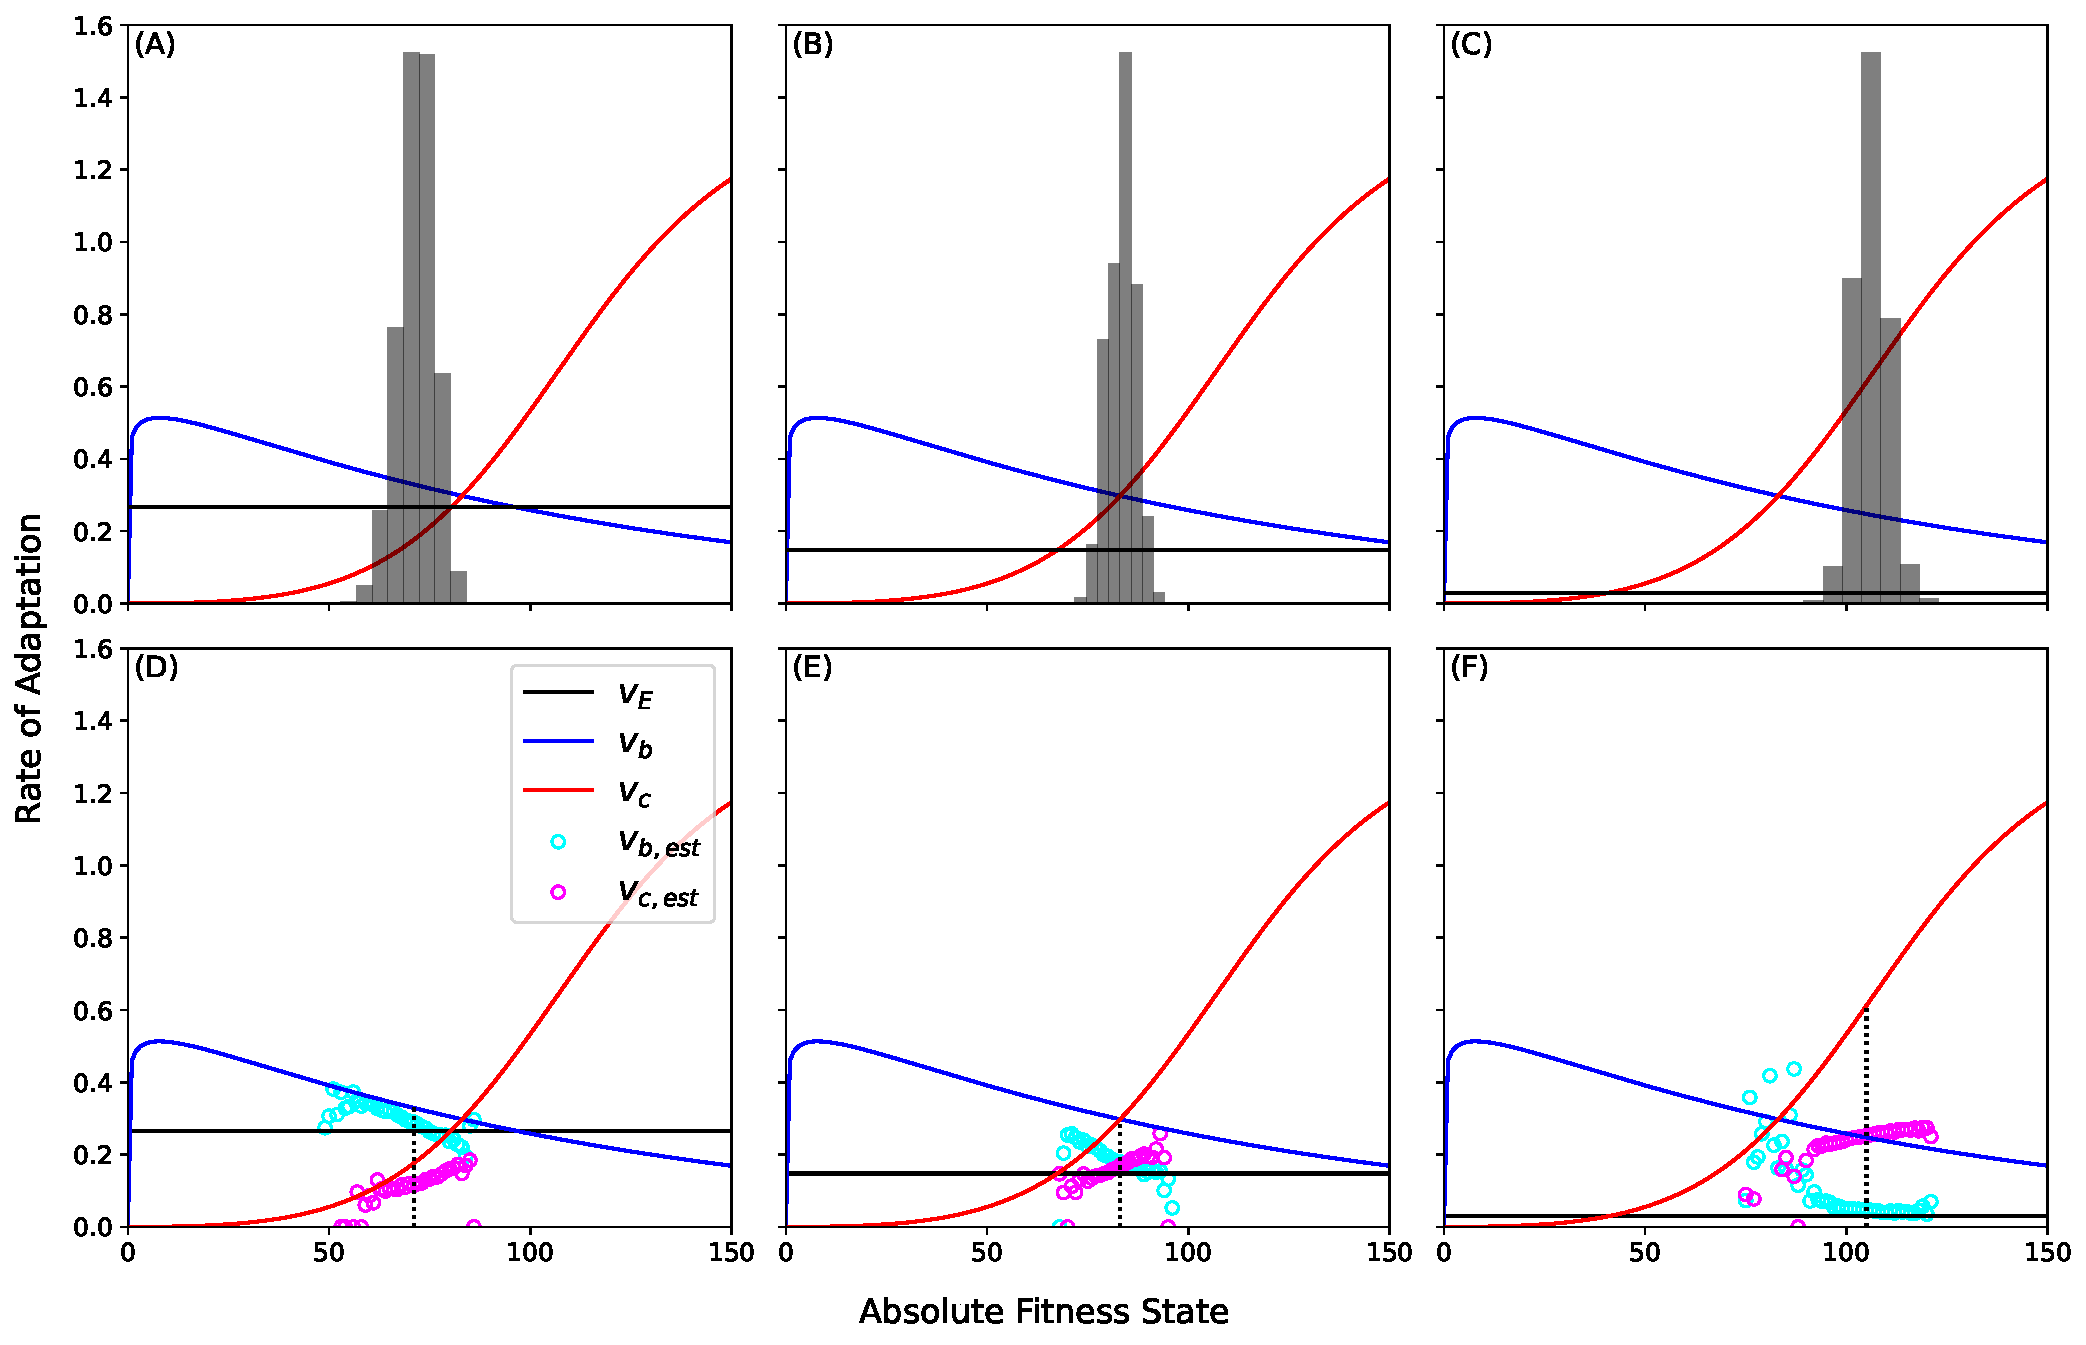
\includegraphics[scale=.51]{Fig/Supplement/fig_bEvo_DRE_traitInterference_mcPlots_pnlC.pdf}
    \caption{Simulations depart least from analytical expectations when $v_E$ equals half the rate of adaptation at the $v_C=v_B$ intersection (middle column). Perfect interference would make both $v_C$ and $v_B$ at the intersection equal to exactly half the values they would be in the absence of interference, as singular values in the middle of a step function at the point of intersection. In simulations of imperfect interference, we see these two rates fall by half as expected, but with transition zones on either side (bottom row, cyan and magenta points), rather than a step function. Simulated populations tend to be found (histograms in top row) at the intersection (bottom row, dashed vertical line) of simulated $v_B$ (cyan) and $v_E$ (black horizontal line). Environmental change at half the analytically expected rate $v_B=v_C$ (panel E) has a halved $v_B$ perfectly balanced both against a halved $v_C$, and against $v_E$, such that the simulated population remains close to the intersection. Deviations from analytical expectations for other $v_E$ values are small in magnitude compared to what one would see with no clonal interference (Supplementary Figure S5). The slow environmental change case (panel F) reveals that our analytical approximation of $s_C$ is an overestimate at high population densities (magenta points, far right, are much lower than red line even after cyan points become small). Cyan and magenta estimates of rates of adaptation are calculated from the sojourn times used to construct histograms in the top row. $v_E$ is set to $90\%$ (A), $50\%$ (B) and $10\%$ (C) of the value corresponding to the $v_b=v_c$ rate of adaptation. $\rho=1.12$ throughout; results for $\rho=0.93$ and $1.0$ were examined and found to be similar. $T=10^9$, $d=1.2$, $U_b=5\times10^{-6}$, $U_c=5\times10^{-6}$, $s_{b,0}=0.02$, $\alpha=0.995$, and $c_{+}=0.02$.}
    \label{fig:supp:stallingTypes}
\end{figure}
\vspace*{\fill}\clearpage
\end{landscape}
\newpage
\vspace*{\fill}
\begin{figure}[!h]
    \centering
    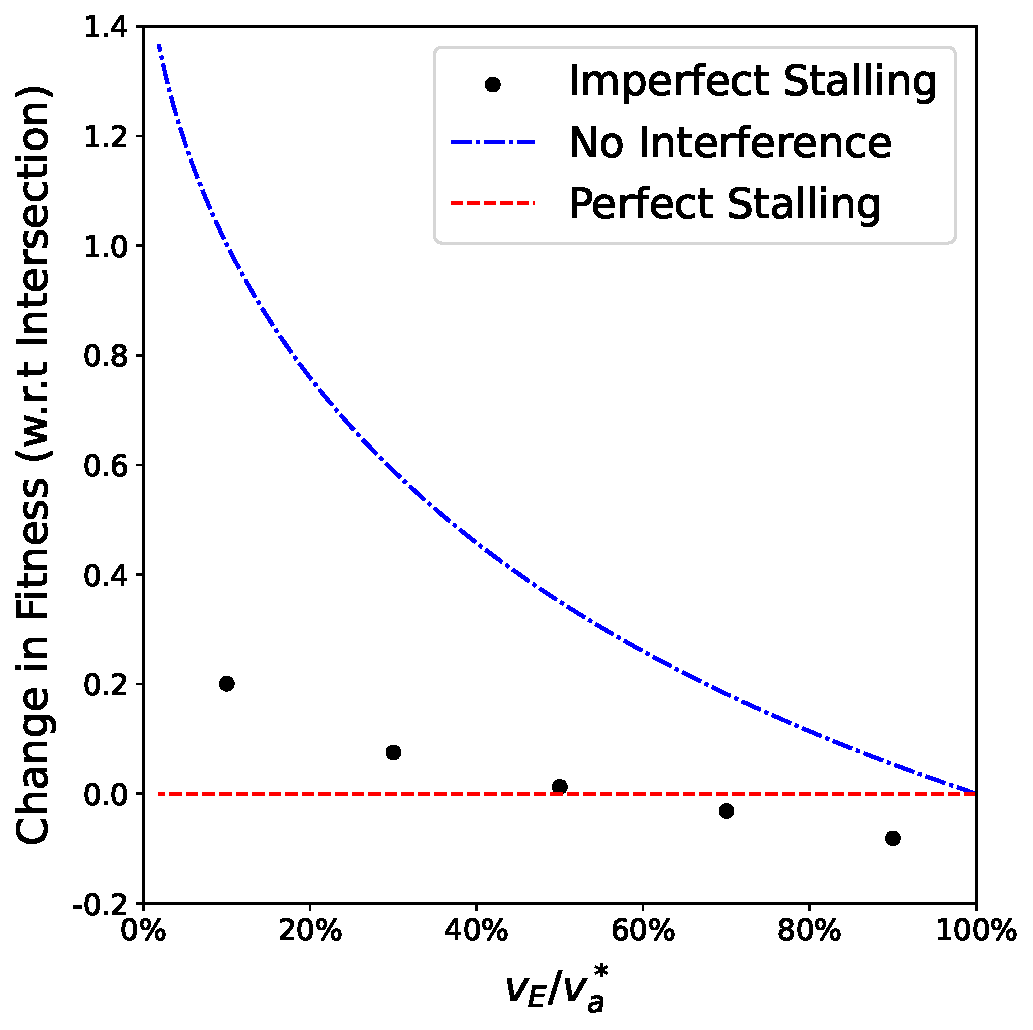
\includegraphics[scale=.62]{Fig/Supplement/fig_bEvo_DRE_traitInterference_fitnessGain_rho1.pdf}
    \caption{The deviations from analytical expected population fitness caused by different values of $v_E$ are small in magnitude compared to what one would see with no clonal interference. Solid points for imperfect stalling reflect mean values of the histograms in Supplementary Figure S4. $T=10^9$, $d=1.2$, $U_b=5\times10^{-6}$, $U_c=5\times10^{-6}$, $s_{b,0}=0.02$, $\alpha=0.993$, and $c_{+}=0.02$.}
\label{fig:supp:stallingTypes_varyVE}
\end{figure}
\vspace*{\fill}\clearpage

\newpage
\vspace*{\fill}
\begin{figure}[!h]
    \centering
    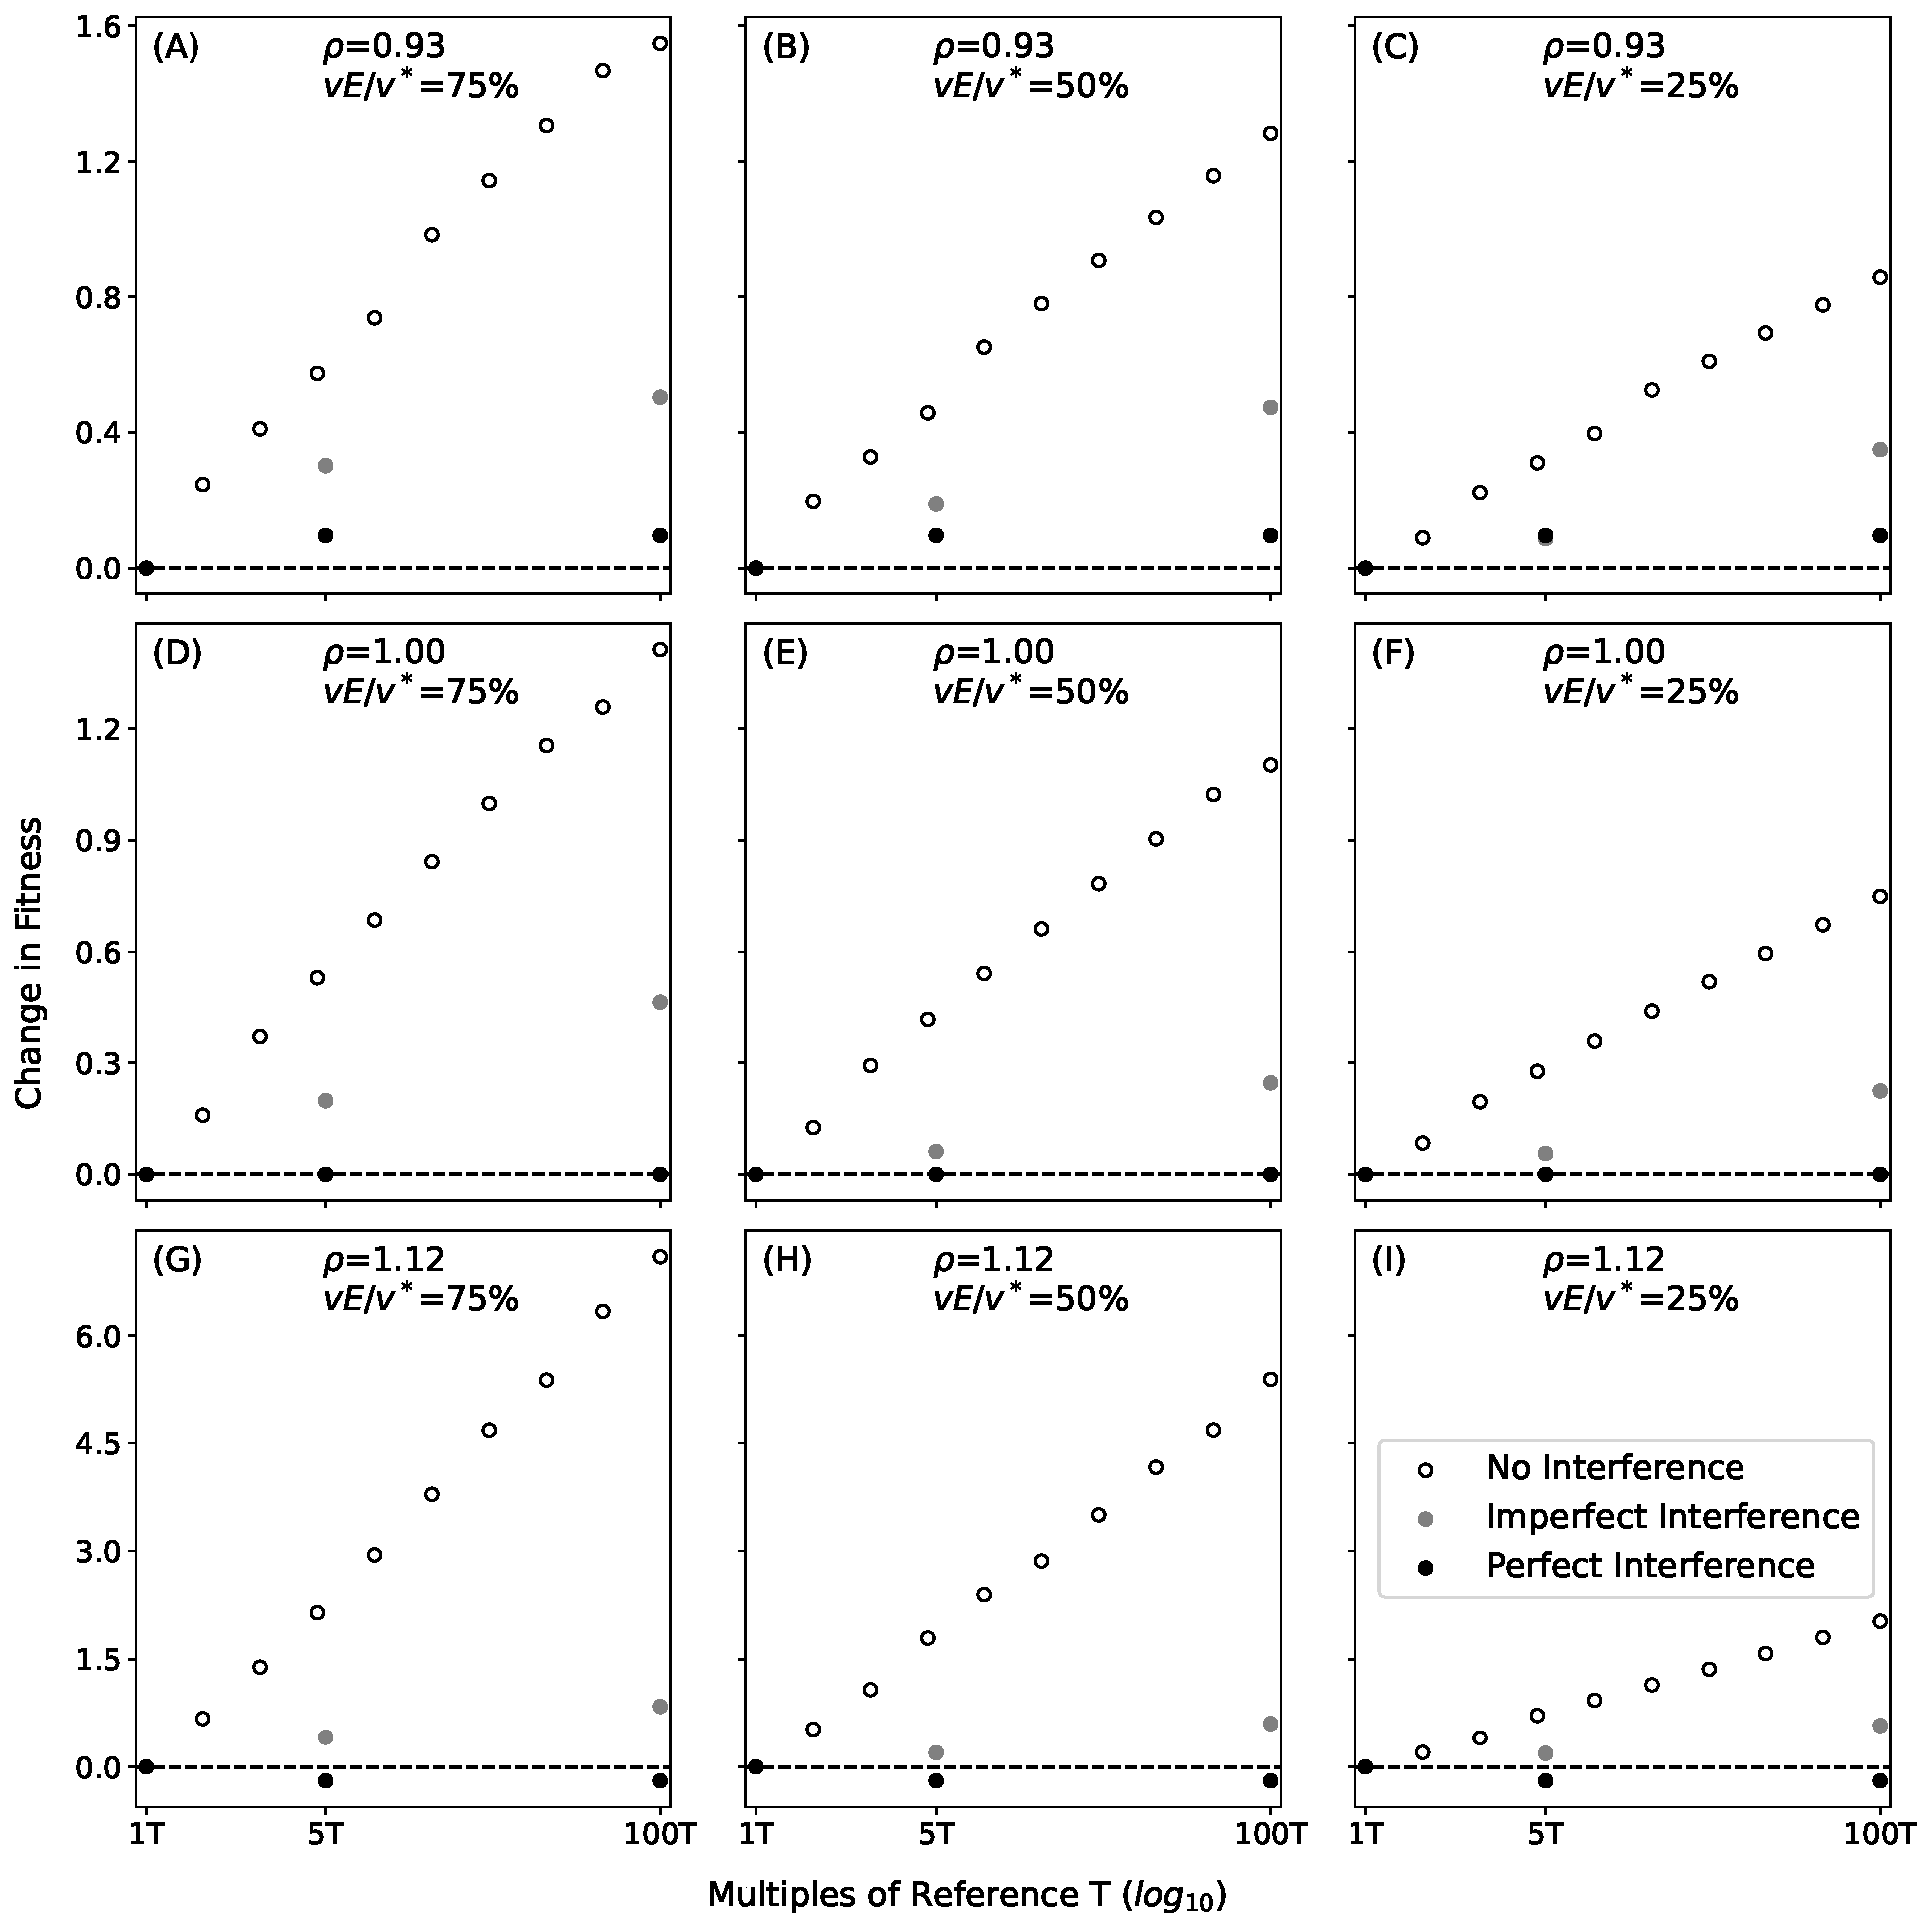
\includegraphics[scale=.5]{Fig/Supplement/fig_bEvo_DRE_traitInterference_increaseT.pdf}\\
    \caption{Simulations confirm that clonal interference eliminates most of the benefit to absolute adaptation that would otherwise come from a larger habitat. Presentation follows that in Figure 4, but with different values of $\rho$ (rows), and of $v_E$ as a fraction of $v^*=v_B=v_C$ (columns); Figure 4 corresponds to panel (H). Simulations are shown in grey, predictions from the intersections of analytic curves in solid black, and results with no evolution in the $c$-trait as open circles. The x-axis shows fold-change in absolute fitness attributable to the increase in $T$ from a starting point of $1T=10^9$. $d=1.2$, $U_c=5\times10^{-6}$, and $c_{+}=0.02$ throughout. For panels (A) through (C), $U_b=5\times10^{-7}$, $s_{b,0}=0.03$, and $\alpha=0.99$. For panels (D) through (F), $U_b=5\times10^{-6}$, $s_{b,0}=0.02$, and $\alpha=0.993$. For panels (G) through (I), $U_b=5\times10^{-6}$, $s_{b,0}=0.02$, and $\alpha=0.995$.}
\label{fig:supp:stallingTypes_varyT}
\end{figure}
\vspace*{\fill}\clearpage

\end{document}


